\documentclass[12pt, a4]{report}
\usepackage[utf8]{inputenc}
\usepackage{fullpage}
\usepackage{hyperref}
\usepackage{graphicx}
\usepackage{titlesec}
\usepackage{custom}

\titleformat{\chapter}[display]{\normalfont\bfseries}{}{0pt}{\Huge}

% Inserting Document Header
\documentheader{USE CASE DOCUMENT}{1.2}{1$^{st}$ May, 2021}

\begin{document}
\maketitle
\newpage
\tableofcontents

% --------------------------------------------------------------------------------------------------

\newpage
\chapter{Use Case Diagram}
The Use Case Diagram proposed for the Online Course Management System, based on the Software Requirements Specification (SRS) Version 1.2 is shown below.
\begin{figure}[h]
    \begin{center}
        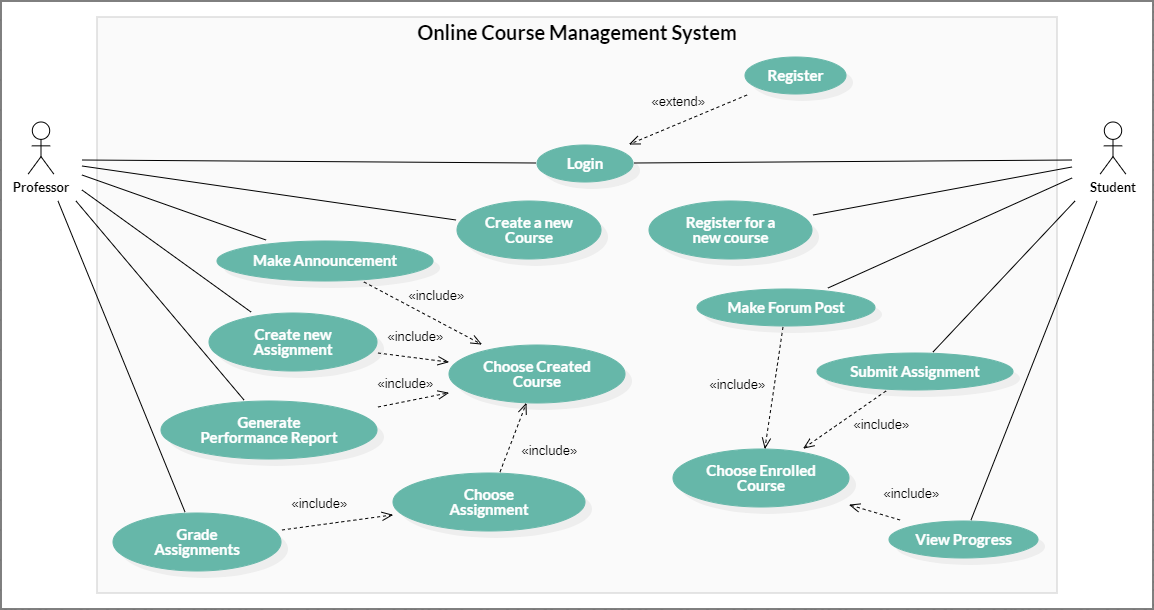
\includegraphics[width=\textwidth]{Diagrams/Use Case Diagram v1.2.png}
        \textsc{Use Case Diagram Version 1.2}
    \end{center}
\end{figure}

% --------------------------------------------------------------------------------------------------
% --------------------------------------------------------------------------------------------------

\newpage
\chapter{Use Case Descriptions}

% --------------------------------------------------------------------------------------------------

\usecase {Login}
{ % Overview
This use case describes how a user (Student, Professor or System Admin) can log into the system to use it
}
{ % Actors
Student, Professor, System Admin
}
{ % Basic Flow
\begin{enumerate}
    \item The user enters their login credentials (Username \& Password).
    \item The system authenticates the user using the internal database.
    \item The user is logged into the system.
\end{enumerate}
}
{ % Alternate Flows
\textbf{The credentials are incorrect}
\begin{enumerate}
    \item The system displays an error message and resets the Login Page.
    \item The user re-initiates the use-case.
\end{enumerate}
}
{ % Pre-Conditions
}
{ % Post-Conditions
The user is successfully logged into the system.
}
{ % Includes
}
{ % Extends
}

% --------------------------------------------------------------------------------------------------

\newpage
\usecase {Register}
{ % Overview
This use case describes how a user (Student, Professor or System Admin) can register an account in the System.
}
{ % Actors
Student, Professor, System Admin
}
{ % Basic Flow
\begin{enumerate}
    \item The user enters their details and a chosen password.
    \item The system adds the user to the database.
    \item The system redirects back to the login page.
\end{enumerate}
}
{ % Alternate Flows
}
{ % Pre-Conditions
The user must not already have an account and should wish to create one in the system.
}
{ % Post-Conditions
The user is successfully registered into the system, and can now login anytime later.
}
{ % Includes
}
{ % Extends
Login
}

% --------------------------------------------------------------------------------------------------

\usecase {Register for a course}
{ % Overview
This use case describes how a Student can register for a course.
}
{ % Actors
Student
}
{ % Basic Flow
\begin{enumerate}
    \item The system displays all available courses.
    \item The student chooses one of the courses.
    \item The system displays the details of the chosen course.
    \item The students confirms registration and the database is updated.
\end{enumerate}
}
{ % Alternate Flows
\begin{enumerate}
    \item The student chooses not to register and goes back to the course catalog.
\end{enumerate}
}
{ % Pre-Conditions
}
{ % Post-Conditions
The student is successfully registered to their chosen course.
}
{ % Includes
}
{ % Extends
}

% --------------------------------------------------------------------------------------------------

\usecase {Choose Enrolled Course}
{ % Overview
This use case describes how a Student can choose to manage a course they are enrolled in.
}
{ % Actors
Student
}
{ % Basic Flow
\begin{enumerate}
    \item The system displays all courses the student has enrolled in.
    \item The student chooses one of the courses.
    \item The system redirects student to the dashboard of the course.
\end{enumerate}
}
{ % Alternate Flows
}
{ % Pre-Conditions
}
{ % Post-Conditions
The dashboard of the chosen course is displayed to the student.
}
{ % Includes
}
{ % Extends
}

% --------------------------------------------------------------------------------------------------

\usecase {Make Forum Post}
{ % Overview
This use case describes how a Student can make a post in the Course Public Forum.
}
{ % Actors
Student
}
{ % Basic Flow
\begin{enumerate}
    \item The student types and sends a message they want to send on the course forum.
    \item The system saves the message to the database and displays it on the forum.
\end{enumerate}
}
{ % Alternate Flows
}
{ % Pre-Conditions
}
{ % Post-Conditions
A forum post is made by the student that can be viewed by other students taking the course as well as the professor that is handling the course.
}
{ % Includes
Choose Enrolled Course
}
{ % Extends
}

% --------------------------------------------------------------------------------------------------

\newpage
\usecase {Submit Assignment}
{ % Overview
This use case describes how a Student can submit an assignment.
}
{ % Actors
Student
}
{ % Basic Flow
\begin{enumerate}
    \item The system displays all assignments pending for the course.
    \item The student chooses one of the assignments.
    \item The system displays all details of the assignment.
    \item The students enters a Google Drive link to their assignment submission.
\end{enumerate}
}
{ % Alternate Flows
}
{ % Pre-Conditions
}
{ % Post-Conditions
The student successfully makes a submission to the assignment.
}
{ % Includes
Choose Enrolled Course
}
{ % Extends
}

% --------------------------------------------------------------------------------------------------

\usecase {View Progress}
{ % Overview
This use case describes how a Student can view their progress in any chosen course.
}
{ % Actors
Student
}
{ % Basic Flow
\begin{enumerate}
    \item The system retrieves scores issued by the professor handling the course.
    \item The assignment scores of the student are displayed.
\end{enumerate}
}
{ % Alternate Flows
}
{ % Pre-Conditions
}
{ % Post-Conditions
}
{ % Includes
Choose Enrolled Course
}
{ % Extends
}

% --------------------------------------------------------------------------------------------------

\newpage
\usecase {Create Course}
{ % Overview
This use case describes how a Professor can create a new course.
}
{ % Actors
Professor
}
{ % Basic Flow
\begin{enumerate}
    \item The professor enters all details relating to the course.
    \item The system creates a new course and adds it to the wait-list for approval by the System Administrator.
\end{enumerate}
}
{ % Alternate Flows
}
{ % Pre-Conditions
}
{ % Post-Conditions
The course is created and students can register for it.
}
{ % Includes
}
{ % Extends
}

% --------------------------------------------------------------------------------------------------

\usecase {Choose Created Course}
{ % Overview
This use case describes how a Professor can choose to manage a course created by them.
}
{ % Actors
Professor
}
{ % Basic Flow
\begin{enumerate}
    \item The system retrieves all courses created by the professor from the database and displays them.
    \item The professor chooses on of the courses.
    \item The system redirects to the dashboard of the course.
\end{enumerate}
}
{ % Alternate Flows
}
{ % Pre-Conditions
}
{ % Post-Conditions
The dashboard of the chosen course is displayed to the professor.
}
{ % Includes
}
{ % Extends
}

% --------------------------------------------------------------------------------------------------

\newpage
\usecase {Make Forum Post}
{ % Overview
This use case describes how a Professor can make a post in the Course Forum.
}
{ % Actors
Professor
}
{ % Basic Flow
\begin{enumerate}
    \item The professor enters the desired post to be made into the forum.
    \item The system creates a forum post and updates the database.
\end{enumerate}
}
{ % Alternate Flows
}
{ % Pre-Conditions
}
{ % Post-Conditions
An announcement is made by the professor on the forum that can be viewed by all students taking the course.
}
{ % Includes
Choose Created Course
}
{ % Extends
}

% --------------------------------------------------------------------------------------------------

\usecase {Create New Assignment}
{ % Overview
This use case describes how a Professor can create a new Assignment and post it.
}
{ % Actors
Professor
}
{ % Basic Flow
\begin{enumerate}
    \item The professor enters the details of the course along with any resource links necessary.
    \item The system creates an assignment activity and posts it in the assignments tab of the course dashboard.
    \item The system also makes an announcement in the forum regarding the assignment.
    \item The assignment will accept submissions from the students taking the course.
\end{enumerate}
}
{ % Alternate Flows
}
{ % Pre-Conditions
}
{ % Post-Conditions
An assignment is created and posted for the students to work on and submit.
}
{ % Includes
Choose Created Course
}
{ % Extends
}

% --------------------------------------------------------------------------------------------------

\newpage
\usecase {Choose Assignment}
{ % Overview
This use case describes how a Professor can choose to manage an assignment.
}
{ % Actors
Professor
}
{ % Basic Flow
\begin{enumerate}
    \item The professor chooses an assignment from the assignments tab.
    \item The system retrieves all information about the assignment and all submissions made by students and displays them for the professor.
\end{enumerate}
}
{ % Alternate Flows
}
{ % Pre-Conditions
}
{ % Post-Conditions
}
{ % Includes
Choose Created Course
}
{ % Extends
}

% --------------------------------------------------------------------------------------------------

\usecase {Grade Assignments}
{ % Overview
This use case describes how a Professor can grade grade submissions made by students to an assignment.
}
{ % Actors
Professor
}
{ % Basic Flow
\begin{enumerate}
    \item The professor chooses an assignment from the assignments tab.
    \item The system retrieves all information about the assignment and all submissions made by students and displays them for the professor.
    \item The professor provides a score for each of the submissions.
    \item The system saves the scores, updates the database and makes a forum post that the respective assignment has been graded along with the list of students whose submissions have been graded.
\end{enumerate}
}
{ % Alternate Flows
}
{ % Pre-Conditions
}
{ % Post-Conditions
}
{ % Includes
Choose Assignment
}
{ % Extends
}

% --------------------------------------------------------------------------------------------------

\newpage
\usecase {Generate Performance report}
{ % Overview
This use case describes how a Professor can generate a performance report for any course handled by them.
}
{ % Actors
Professor
}
{ % Basic Flow
\begin{enumerate}
    \item The system retrieves all assignment scores of students enrolled in the course.
    \item The system generates a report of their performances and displays it to the professor.
\end{enumerate}
}
{ % Alternate Flows
}
{ % Pre-Conditions
}
{ % Post-Conditions
}
{ % Includes
Choose Created Course
}
{ % Extends
}

% --------------------------------------------------------------------------------------------------

\end{document}